\def\ChapterTitle{Background on Trust and its Applications to \gls{manet}s} % Write in your own chapter title
\ifx\ifthesis\undefined
\documentclass[a4paper, 11pt]{article}

% % Special Includes stolen from Thesis.cls
\usepackage{booktabs}
\usepackage{hyperref}
\usepackage{graphicx}
\usepackage{epstopdf}
\usepackage{subcaption}
\usepackage{rotating}
\usepackage{listings}
\usepackage{lstpatch}
\renewcommand{\arraystretch}{1.3}

% % % % % % % % % % % % % % % %

% PACKAGES
\usepackage[square, numbers, comma, sort&compress]{natbib}  % Use the "Natbib" style for the references in the Bibliography
\usepackage{verbatim,listings}  % Needed for the "comment" environment to make LaTeX comments
\usepackage{array}  % Needed for the "comment" environment to make LaTeX comments
\usepackage{vector}  % Allows "\bvec{}" and "\buvec{}" for "blackboard" style bold vectors in maths
\usepackage{amsmath,amsfonts,amsthm,color,psfrag,epsf, tabularx, multirow, longtable}
\usepackage{snapshot, todonotes}
% \usepackage{pstricks}
\usepackage{enumerate}
%\usepackage[lined,algonl,boxed]{algorithm2e}
\usepackage[ruled,linesnumbered,vlined]{algorithm2e}
\usepackage{float}
\usepackage{epigraph} % epigraph
\usepackage{tikz}
\usetikzlibrary{shapes.geometric, arrows}

\usepackage{setspace}
\doublespacing
% or:
%\onehalfspacing

% SETUP
\hypersetup{urlcolor=blue, colorlinks=false}  % Colours hyperlinks in blue, but this can be distracting if there are many links. 
\DeclareGraphicsExtensions{.pdf,.jpeg,.png}
\graphicspath{{../Figures/}{../../../Dropbox/Thesis_Figures/}}  % Location of the graphics files (set up for graphics to be in PDF format)

% NOTE THERES A FUCKUP IN TEX4HT http://tug.org/pipermail/tex4ht/2014q2/000944.html
% NEED TO MANUALLY CHANGE \def\pgfsys@svg@newline{{?nl}}
\ifdefined\HCode
\usepackage[compatibility=false]{caption}
\def\pgfsysdriver{pgfsys-tex4ht.def}
\else
\usepackage[]{caption}
\fi

% \SpecialCoor
\def\subsum{\mathit{\Sigma}}

%opening
\title{\ChapterTitle}
\author{Andrew Bolster}

\begin{document}

\maketitle

\else
\chapter{\ChapterTitle}
\label{Chapter\thechapter}
\lhead{Chapter \thechapter.
\emph{\nameref{Chapter\thechapter}}} % Write in your own chapter title to set the page header
\fi
\section{Trust Definitions and Perspectives}
For a term that is so common in every-day speech, Trust is a challenging discussion area, particularly given the wealth of proposed definitions (Table~\ref{tab:trust_definitions})\todo{More of these in the bookmarks list}.
Beyond these dry, vague, and often ``fuzzy'' definitions, there is a significant ontological conflict between the subjective and objective perspectives of trust; is ``trust'' an attribute of the actor performing a given action, or of the observer of such an action? Or indeed is trust itself an action upon a relationship between actors? Is it qualitative or quantitative? These questions have challenged philosophers, psychologists and social scientists for decades.

In human trust relationships it is recognized that there can be several domains of Trust for example organizational, sociological, interpersonal, psychological and neurological \cite{Lee2004}.

These domains of trust are, from a human perspective, quite natural and are formed during the earliest stages of linguistic integration.
This leads to recognisable deviations in the experiential concept of ``trust'' across cultures with differing linguistic histories.
This has led to a wealth of work in the social sciences (as well as management schools across the world) in to how to develop, understand, and repair trust across cultural boundaries.\cite{Okumura2011} \todo{Get more citations for this paragraph, need background on multicultural definitions rather than second hand}
\begin{table}\centering
  \caption{Definitions of Trust}
  \label{tab:trust_definitions}
  \begin{tabularx}{\textwidth}{X p{3cm}}\toprule
    Definition & Source \\ \midrule
    Assured reliance on the character, ability, strength, or truth of someone or something.
    & Merriam-Webster\\
    Firm belief in the reliability, truth, or ability of someone or something & OED\\
    The willingness of a party to be vulnerable to the actions of another party based on the expectation that the other will perform a articular action important to the trustor, irrespective of the ability to monitor or control that other party & \cite{Mayer1995} \\
    An expectancy held by and individual or a group that the word, promise, verbal or written statement of another individual or group can be relied upon & \cite{Rotter1967}\\\bottomrule
  \end{tabularx}
\end{table}
\subsection{Modelling of Trust Relationships}
Mayer et al \cite{Mayer1995} proposed a model of trust that encapsulates generalised factors of perceived trustworthiness in interpersonal relationships (Table~\ref{tab:trust_factors}), accommodating a subjective trustworthiness and risk-taking potentiality on the part of the trustor.
This formulation of trust allowed a wider discussion of the characteristics of trust relationships, both between individuals and within networks or communities.

\begin{table}\centering
  \caption[Factors of Trust]{Factors of Trust\cite{Mayer1995}}
  \label{tab:trust_factors}
  \begin{tabularx}{\textwidth}{p{2cm}X}\toprule
    Factor & Definition \\ \midrule
    Ability & Collection of skills, competencies, capabilities and characteristics that enable a party to have influence or action within some specific domain \\
    Benevolence & The extent to which a trustee is believed to want to do good to or by the trustor beyond a selfish profit motive\\
    Integrity & Acceptance or adherence to a common set of principals of operation that the trustor finds acceptable\\
    \bottomrule
  \end{tabularx}
\end{table}

\begin{figure}
  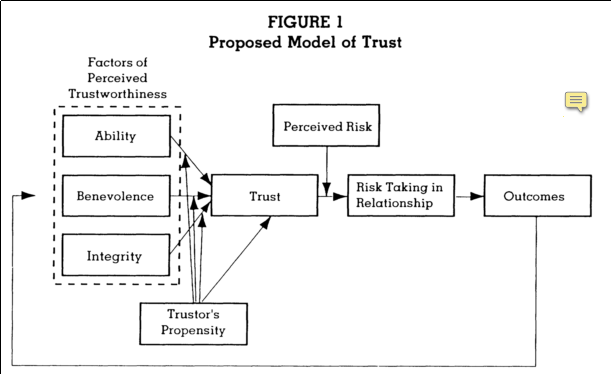
\includegraphics[width=\textwidth]{mayer1995-fig1}
  \caption[Model of Trust]{Model of Trust \cite{Mayer1995}}
  \label{fig:mayer_trust_model}
\end{figure}
Lee and See \cite{Lee2004} extended and synthesised Mayer et al's approach to personal and interpersonal trust towards a generalised concept of trust for human and autonomic/autonomous systems with the following alternative contextual definitions (including their approximate mappings to Mayer et al's approach
\begin{table}
  \caption[Factors of Trust for Autonomous Systems]{Factors of Trust for Autonomous Systems\cite{Lee2004}}
  \label{tab:autonomous_trust_factors}
  \begin{tabularx}{\textwidth}{p{2cm}X p{2cm}}\toprule
    Factor & Definition & Mayer Term\\ \midrule
    Performance & `The current and historical operation of the automation, including characteristics such as reliability, predictability, and ability & Ability\\
    Process & The degree to which the automation's algorithms are appropriate for the situation and able to achieve the operators goals.
    & Integrity\\
    Purpose & The degree to which the automation is being used within the realm of the designers intent & Benevolence \\
    \bottomrule
  \end{tabularx}
\end{table}


\subsection{Characteristics of Trust Relationships}

There are five commonly considered characteristics or attributes of Trust relationships in general, but not all relationships exhibit them and they are not assumed to be a complete specification of Trust:

\begin{itemize}
  \item \emph{Multi-Party} - One-to-one; one-to-many; many-to-one; many-to-many.
    Trust is not an absolute characteristic of a lone individual.
    Trust may include multi-agent abstractions (one-to-many), such as a preferential trust/distrust towards a group exhibiting a particular attribute, e.g.\ members of the armed forces / police services.
    Likewise, there can be trustor/trustee attributes that can generalise relationships between collectives (many-to-many), e.g.\ Jets and Sharks
  \item \emph{Transitive} - Trust assessments can be shared (i.e.\ recommendations), where this second order trust assessment incorporates both the observed trustworthiness of the trustee, as well as the trustworthiness of the intermediate trustor.
    In some models this is further extended to include out-of-network intermediate trustors that have some other defined authority, e.g.\ PKI Certificate Authority
  \item \emph{Evidential} - Trust must be based on some form of evidence-based observation or assessment, such as historical success rates of performing a certain action, or second-hand observations of trust from a third party.
  \item \emph{Directional Asymmetry} - The majority of relationships are bi-directional but are asymmetric, i.e.\ between two entities who ``trust'' each other, there are two independent trust relationships that may have very different ``values'' or extents.
  \item \emph{Contextual} - Trust can be variable and loosely coupled between contexts with respect to the action being assessed or the environment within which the trustee is operating, e.g.
    Doctors are trusted to perform medical procedures but that trust may not improve their success at correctly wiring an electrical plug.
    However there are plenty of counter-examples to this, as from \cite{Mayer1995}, two of the three listed factors of trust are ``Benevolence'' and ``Integrity'' and are unrelated to the ability of a trustee to perform a particular action, so it is reasonable to make an initial assumption that if a trustee is being benevolent in one activity or context, that that benevolence \emph{should} extend to other contexts.

\end{itemize}
\subsection{Topologies of Trust Networks}
\label{sec:trust_topologies}
Beyond the attributes or characteristics of an individual trust relationship, within any multi party sparsely connected network or community, topological context is useful in both establishing trust and in disseminating observations for collaborative assessment.

\missingfigure{Trust Topologies, Direct, Indirect, Recommender, etc.
We've done it a dozen times before, may as well make a new graphic}

\section{Trust in \gls{manet}s}
\subsection{Trust Perspectives in Autonomous Operation}
For the purposes of this work we define two perspectives on trust for autonomous systems: Design and Operational.
These are summarised in Table~\ref{tab:trust_perspectives}.
It is useful to further define and classify Operational Trust into two distinct but related sections defined in Table~\ref{tab:operational_trust_perspectives}.\todo{Work out how to reference across chapters in a multi doc}
\begin{table}
  \begin{tabularx}{\textwidth}{p{3cm}X}\toprule
    \emph{Design Trust} & When an autonomous system is under development a level of Trust is established in it through the manner in which it has been designed and tested.
    This is the same as conventional systems.\par
    Given that systems that have high-levels of autonomy are designed to behave adaptively to dynamic environments, it is challenging to fully predict such non-deterministic behaviours prior to operational deployment.
    For example, in a navigation system it is difficult to predict the dynamic environment it will need to adapt to.\par
    Trust needs to be developed that the design and test of such systems are sufficient to predict that operation will be, if not optimal, at least satisfactory.
    \\
    \emph{Operational Trust} & Trust at runtime or in-situ that both the individual nodes within a system are operating as expected and that the interfaces between the operator and the system are as expected.
    \par
    This latter aspect covers issues such as physical/wireless links and interpretation of data at each end of such a communication link.
    Operational Trust is functionally derived from, but distinct from Design Trust.\\
    \bottomrule
  \end{tabularx}
  \caption{Trust Perspectives with respect to autonomous systems}
  \label{tab:trust_perspectives}
\end{table}
\begin{table}
  \begin{tabularx}{\textwidth}{p{3cm}X}\toprule
    \emph{Hard Trust} or technical trust & The quantitative measurement and communication of the expectation of an actor performing a certain task, based on historic performance and through consensus building within a networked system.\par
    Can be thought of as a de-risking strategy to measure and monitor the ability of a system, or another actor within a system, to perform a task unsupervised.\\
    \emph{Soft Trust} or common trust & The qualitative assessment of the ability of an actor to perform a task or operation consistently and reliably based on social or experiential factors.\par
    This is the ‘human’ form of trust and is the main motivational driver for the human-factors trust discussion in *OTHER CHAPTER*.\par
    Can be rephrased as the level of confidence an operator has in an actor to perform a task unsupervised.\\
    \bottomrule
  \end{tabularx}
  \caption{Trust Perspectives within Operational Trust}
  \label{tab:operational_trust_perspectives}
\end{table}

It is already clear that these two definitions are extremely close in their construction, but represent fundamentally different approaches to trust, one coming from a sociological perspective of person-to-person and person-to-group relationships from day to day life, and the other coming from a statistical or formal appraisal of an activity by a system.
For the purposes of this work, we are concerned with the analytical establishment of hard trust within a topologically dynamic network of autonomous actors.

\subsection{Levels of Trust}
\todo{This section may be superfluous}
Trust relationships operate as part of a system architecture, and can quite often get confused.
Sun\cite{Sun2008} suggests that within these there are two overarching forms of trust:
\begin{itemize}
  \item Behavioural: That one entity voluntarily depends on another entity in a specific situation
  \item Intentional: That one entity would be willing to depend on another entity
\end{itemize}
These concepts closely mirror the previous definitions of ‘Hard’ and ‘Soft’ trust respectively, one (Behavioural) being an invested dependency given certain parameters being satisfied, mirroring Hard Trust, and the other (Intentional) being the ‘capacity for belief’ in another entity, analogous to Soft Trust.
It is suggested that these overarching forms are supported by and indeed are drawn from four major constructs within social and networked environments:
\begin{itemize}
  \item Trusting Belief: the subjective belief within a system that the other trusted components are willing and able to act in each-others’ best interests
  \item Dispositional Trust: a general expectation of trustworthiness over time 
  \item Situational Decision Trust: in-situ risk assessment where the benefits of trust outweigh the negative outcomes of trust
  \item System Trust: the assurance that formal impersonal or procedural structures are in place to ensure successful operation.
\end{itemize}
Sun argues that only System Trust and Behavioural Trust are relevant to trusted networking applications.
However, it is arguable that in any network where the operation of that network is not the only concern, or where that network has to interact with any operator, then all of these factors come into play.
Both System and Behavioural trust rely on what Sun calls a ‘Belief Formation Process’, or a trust assessment, while the other trust constructs deal with the interactions between trust and decision making against an internal assessment of network trustworthiness.

\subsection{Trust Model Design Considerations}
Trust is the level of confidence one agent has in another to perform a given action on request or in a certain context.
Trust in the autonomous or semi-autonomous realm is the ability of a system to establish and maintain confidence in itself or another systems' operations.
Managing this trust can be used to predict and reason on the future interactions between entities in a system, such as an autonomous mobile ad-hoc network (\gls{manet}).

The distributed and dynamic nature of \gls{manet}s mean that it is difficult to maintain a trusted third party (TTP) or evidence based trust system such as Certificate Authorities or using Public Key Infrastructures (PKI).\todo{possibly worthwhile doing more background on the operation of these}
Therefore, a distributed, collaborative system must be applied to these networks.
Such distributed trust management frameworks aim to detect, identify, and mitigate the impacts of malicious actors by distributing per-node assessments and opinions to collectively self-police behaviour.

As mobile ad-hoc networks (\gls{manet}s) grow beyond the terrestrial arena, their operation and the protocols designed around them must be reviewed to assess their suitability to different communications environments, ensuring their continued security, reliability, and performance.

Trust Management Frameworks (TMFs) provide information to assist the estimation of future states and actions of nodes within networks.
This information is used to optimize the performance of a network against malicious, selfish, or defective misbehaviour by one or more nodes.
Previous research has established the advantages of implementing TMFs in 802.11 based \gls{manet}s, particularly in terms of preventing selfish operation in collaborative systems \cite{Li2007}, and maintaining throughput in the presence of malicious actors \cite{Buchegger2002}
There are five topics that are important to address in any \gls{manet}s trust model \cite{Kamvar2003}:
\begin{itemize}
  \item The trust model should be without infrastructure.
    Because the network routing infrastructure is formed in an ad-hoc fashion, the trust management can not depend on, e.g., a trusted third party (TTP).
    There is no public key infrastructure (PKI), where some center nodes monitor the network, and publish illegal nodes periodically.
    In a \gls{manet}, there are no certification authorities (CA) or registration authorities (RA) with elevated privileges etc.
  \item The trust model should be anonymous because of the anonymity of mobile nodes in \gls{manet}s.
  \item The trust model should be robust.
    That is, it can be robust to all kinds of unfriendly attacks and the network itself should not be susceptible to attacks by unfriendly nodes.
    Moreover, in the presence of malicious nodes, they may attempt to subvert the model in order to get the unfairly good trust value.
  \item The trust model should have minimal control overhead in accordance with computation, storage, and complexity.
  \item The trust model should be self-organized.
    \gls{manet}s are characterized to have dynamic, random, rapidly changing and multi-hop topologies composed of variably bandwidth-constrained links
\end{itemize}
\section{Current Trust Management Frameworks}
Distributed trust management frameworks for \gls{manet}s aim to detect, identify, and mitigate the impacts of malicious actors by distributing per-node assessments and opinions to collectively self-police behaviour.
Various models and algorithms for describing trust and developing trust management in distributed systems, P2P communities or wireless networks have been considered.
Taking some examples;
\begin{itemize}
  \item \emph{Hermes Trust Establishment Framework} takes a Bayesian Beta function to model per-link Packet Loss Rate (PLR) over time, combining ``Trust'' and ``Confidence of Assessment'' into a single value \cite{Zouridaki2005}.
  \item \emph{The Objective Trust Management Framework} takes a Bayesian approach and introduces the idea of applying a Beta function to changes in the per-link Packet Loss Rate (PLR) over time, combining ``Trust'' and ``Confidence of Assessment'' into a single value \cite{Li2008}.
    \acrshort{otmf} however does not appropriately combat multi-node-collusion in the network \cite{Cho2011}.
  \item \emph{Trust-based Secure Routing \cite{Moe2008a}} demonstrated an extension to Dynamic Source Routing (DSR), incorporating a Hidden Markov Model of the wider ad-hoc network, reducing the efficacy of Byzantine attacks, particularly black-hole attacks but is limited by focusing on single metric observation (PLR)\cite{Cho2011}.
  \item \emph{CONFIDANT}; \cite{Buchegger2002} presented an approach using a probabilistic estimation of normal observations, similar to \acrshort{otmf}.
    They also introduced a greedy topology weighting scheme that internally weighted incoming trust assessments based on historical experience of the reporter.
  \item \emph{Fuzzy Trust-Based Filtering}; \cite{Luo2008} presented a method using Fuzzy Inference to cope with imperfect or malicious recommendation based on a probabilistic estimation of performance using conditional similarity to classify performance using overlapping Fuzzy Set Membership functions to collaboratively filter reputations across a network.
  \item \emph{Multi-parameter Trust Framework for \gls{manet}s (\acrshort{mtfm})} uses a number of communications metrics together for form a vector of trust, apply grey information theory to allow a system to detect and identify the tactics being used to undermine or subvert trust\cite{Guo11}
\end{itemize}
\subsection{Single Metric Trust Frameworks}
\todo{Expand background detail on more frameworks}
The Hermes trust establishment framework \cite{Zouridaki2005} uses Bayesian reasoning to generate a posterior distribution function of ``belief'', or trust, given a sequence of observations of that behaviour, $p(B|O)$\eqref{eq:otmf_pbo}.

\begin{equation}
  p(B|O)  = \frac{p(O|B) \times p(B)}{\rho}
  \label{eq:otmf_pbo}
\end{equation}
Where $p(B)$ is the prior probability density function for the expected normal behaviour, and $\rho$ is a normalising factor.
Due to it's flexibility and simplicity, Hermes assumes that $p(B)$ is a Beta function, and therefore the evaluation of this trust assessment is based around the expectation value of the distribution \eqref{eq:otmf_t}  where $\alpha$ and $\beta$ represent the number of successful and unsuccessful interactions respectively for a particular node $i$.

A secondary measurement of the confidence factor of the trust assessment $t$ is generated as \eqref{eq:otmf_c} and these measurements are combined to form a ``trustworthiness'' value $T$ \eqref{eq:otmf_trust}.

\begin{align}
  t_i &\to E\lbrack\text{beta}(p|\alpha,\beta)\rbrack = \frac{\alpha_i}{\alpha_i+\beta_i} \label{eq:otmf_t}\\[5pt]
  c_i &= 1 - \sqrt{\frac{12\alpha_i\beta_i}{(\alpha_i+\beta_i)^2(\alpha_i+\beta_i+1)}} \label{eq:otmf_c}\\[5pt]
  T_i &= 1 - \frac{\sqrt{\frac{(t_i-1)^2}{x^2} + \frac{(c_i-1)^2}{y^2}}}{\sqrt{\frac{1}{x^2}+\frac{1}{y^2}}} \label{eq:otmf_trust}
\end{align}
In \eqref{eq:otmf_trust}, $x$ and $y$ are constants, used weight the two-dimensional polar mapping of trust and confidence assessments ($t_i,c_i$), and from \cite{Zouridaki2005}, are taken as $x=\sqrt{2},y=\sqrt{9}$.

Upon this per-node assessment methodology, \acrshort{otmf} overlays an observation distribution protocol so as to make the measurements $\alpha_i$ and $\beta_i$ representative of the direct and 1-hop networks observations of the target node $i$, as well as expiring old observations from assessment and eliminating observations from ``untrustworthy'' nodes.

\todo{Want at least CONFIDANT and Fuzzy in here for contrast}
To date this work has been mostly limited to terrestrial, RF based networks.
There are also situations where the observed metrics will include significant noise and occur at irregular, sparse, intervals.
Conventional approaches such as probabilistic estimation do not produce trust values that reflect the underlying reality and context of the metrics available, as they require a-priori assumption that the trust value under exploration has an expected distribution, that distribution is mono-modal, and the input metrics are binary.
In scenarios with variable, sparse, noisy metrics, estimating the distribution is difficult to accomplish a-priori.

Hermes, \acrshort{otmf}, CONFIDANT, and Fuzzy Trust-Based Filtering can be generalised as single-value probabilistic estimation, based on a Bayesian idea of taking a binary input state and generating an idealised Beta Distribution (\ref{eq:beta}) of the future states of that input generated through an expectation value based on interactions (\ref{eq:beta_e}).
\begin{align}
  \label{eq:beta}
  \text{beta}(p|\alpha,\beta) = \frac{\Gamma(\alpha + \beta)}{\Gamma(\alpha)\Gamma(\beta)}p^{\alpha-1},\text{where } 0 \leq p \leq 1; \alpha,\beta > 0\\
  \label{eq:beta_e}
  E(p) = \frac{\alpha}{\alpha + \beta}
\end{align}
Where $\alpha$ and $\beta$ represent the number of successful and unsuccessful interactions respectively.

These single metric TMFs provide malicious actors with a significant advantage if their activity is undetectable by that one assessed metric, especially if the attacker is aware of the observed metric in advance.

The objective of operating a TMF is to increase the confidence in, and efficiency of, a system by reducing the amount of undetectable negative operations an attacker can perform.
In the case where the attacker can subvert the TMF, the metric under assessment by that TMF does not cover the threat mounted by the attacker.
In turn, this causes a super-linearly negative effect in the efficiency of the network as the TMF is assumed to have reduced the possible set of attacks when in fact it has only made it more advantageous to attack a different aspect of the networks operation.
An example of such a behaviour would be the case in a TMF focused on PLR where an attacker selectively delays packets going through it, reducing the over all throughput of one or more virtual network routes.
Such behaviour would not be detected by the TMF.

\subsection{Multi-Metric Trust Frameworks}\label{sec:multimetrictrust}
Given the potential incentives to a selfish attacker and potential threats to trust and fairness in sparse, noisy, and constrained environments, single metric trusts discussed above do not suitably cover the exposed threat surface.\todo{Probably best to just send a reference forward to the Marine Comms chapter}
A multi-metric approach may be more appropriate to capture and monitor the realities of harsh and sparse communications environments.

\acrshort{mtfm}\cite{Guo11} uses Grey Theory\cite{Zuo1995} to perform cohort based normalization of metrics at runtime, providing a ``grey relational grade'' of trust compared to other observed nodes in that interval for individual metrics, while maintaining the ability to reduce trust values down to a stable assessment range for decision support without requiring every environment entered into to be characterised.
This presents a stark difference between the Grey and Probabilistic approaches.
Grey assessments are relative in both fairly and unfairly operating networks.
All nodes will receive mid-range trust assessments if there are no malicious actors as there is nothing ``bad'' to compare against, and variations in assessment will be primarily driven by topological and environmental factors.
Guo et al.\cite{Guo11} demonstrated the ability of grey relational analysis (GRA) to normalise and combine disparate traits of a communications link such as instantaneous throughput, received signal strength, etc.\ into a grey relational coefficient (GRC), or a ``trust vector'' in this instance.

The grey relational vector is given as
%
\begin{align}
  \label{eq:grc}
  \theta_{k,j}^t = \frac{\min_k|a_{k,j}^t - g_j^t| + \rho \max_k|a_{k,j}^t-g_j^t|}{|a_{k,j}^t-g_j^t| + \rho \max_k|a_{k,j}^t-g_j^t|} \\
  \phi_{k,j}^t = \frac{\min_k|a_{k,j}^t - b_j^t| + \rho \max_k|a_{k,j}^t-b_j^t|}{|a_{k,j}^t-b_j^t| + \rho \max_k|a_{k,j}^t-b_j^t|} \notag 
\end{align}
%
where $a_{k,j}^t$ is the value of an observed metric $x_j$ for a given node $k$ at time $t$, $\rho$ is a distinguishing coefficient set to $0.5$, $g$ and $b$ are respectively the ``good'' and ``bad'' reference metric sequences from $\{a_{k,j}^t k=1,2\dots K\}$, i.e.\ $g_j=\max_k({a_{k,j}^t})$,  $b_j=\min_k({a_{k,j}^t})$ (where each metric is selected to be monotonically positive for trust assessment, e.g.\ higher throughput is presumed to be always better).

Weighting can be applied before generating a scalar value \eqref{eq:metric_weighting} allowing the detection and classification of misbehaviours.

%
\begin{equation}
  \label{eq:metric_weighting}
  [\theta_k^t, \phi_k^t] = \left[\sum_{j=0}^M h_j \theta_{k,j}^t,\sum_{j=0}^M h_j \phi_{k,j}^t \right]
\end{equation}
%
Where $H=[h_0\dots h_M]$ is a metric weighting vector such that $\sum h_j = 1$, and in unweighted case, $H=[\frac{1}{M},\frac{1}{M}\dots\frac{1}{M}]$.
$\theta$ and $\phi$ are then scaled to $[0,1]$ using the mapping $y = 1.5 x - 0.5$.
To minimise the uncertainties of belonging to either best ($g$) or worst ($b$) sequences in \eqref{eq:grc} the $[\theta,\phi]$ values are reduced into a scalar trust value by $T_k^t = ({1+{(\phi_k^t)^2}/{(\theta_k^t)^2}})^{-1}$ \cite{Hong2010}.
\acrshort{mtfm} combines this GRA with a topology-aware weighting scheme \eqref{eq:networkeffects} and a fuzzy whitenization model \eqref{eq:whitenization}.

There are three classes of topological trust relationship used; Direct, Recommendation, and Indirect, repeating those discussed in section~\ref{sec:trust_topologies}.\todo{This is currently half empty}
Where an observing node $n_i$ assesses the trust of another target node, $n_j$; the Direct relationship is $n_i$'s own observations $n_j$'s behaviour.
In the Recommendation case, a node $n_k$ which shares Direct relationships with both $n_i$ and $n_j$, gives its assessment of $n_j$ to $n_i$.
In the Indirect case, similar to the Recommendation case, the recommender $n_k$ does not have a direct link with the observer $n_i$ but $n_k$ has a Direct link with the target node, $n_j$.
These relationships give node sets, $N_R$ and $N_I$ containing the nodes that have recommendation or indirect, relationships to the observing node respectively.
%
\begin{align}
  \label{eq:networkeffects}
  T_{i,j}^{\acrshort{mtfm}}=&\frac{1}{2} \cdot \max_s\{f_s(T_{i,j})\} T_{i,j}\\ \notag
  +&\frac{1}{2} \frac{2|N_R| }{2|N_R| + |N_I|}\sum_{n \in N_R} \max_s\{f_s(T_{i,n})\} T_{i,n}\\ \notag
  +&\frac{1}{2} \frac{|N_I| }{2|N_R| + |N_I|}\sum_{n \in N_I} \max_s\{f_s(T_{i,n})\} T_{i,n} 
\end{align}
Where $T_{i,n}$ is the subjective trust assessment of $n_i$ by $n_n$, and $f_s = [ f_1,f_2, f_3]$ given as:
\begin{align}
  \label{eq:whitenization}
  f_1(x)&= -x+1\notag\\
  f_2(x)&= 
  \begin{cases}
    2x & \text{if }x\leq 0.5\\
    -2x+2 & \text{if }x>0.5
  \end{cases}\\
  f_3(x)&= x\notag
\end{align}
%
In the case of the terrestrial communications network used in \cite{Guo11}, the observed metric set $X = {x_1,\dots,x_M}$ representing the measurements taken by each node of its neighbours at least interval, is defined as $X=[$packet loss rate, signal strength, data rate, delay, throughput$]$.

Guo et al.\ demonstrated that when compared against \acrshort{otmf} and Hermes trust assessment, \acrshort{mtfm} provided increased variation in trust assessment over time, providing more information about the nodes' behaviours than packet delivery probability alone can.

\section{Grey System Theory and Grey Trust Assessment}
\todo{This section largely repeats from \acrshort{mtfm} discussion but the maths needs explored somewhere}
\subsection{Grey numbers, operators and terminology}
Grey numbers are used to represent values where their discrete value is unknown, where that number may take its possible value within an interval of potential values, generally written using the symbol $\oplus$.
Taking $a$ and $b$ as the lower and upper bounds of the grey interval respectively, such that $\oplus \in [a,b] | a < b$ 
The ``field'' of $\oplus$ is the value space $[a,b]$.
There are several classifications of grey numbers based on the relationships between these bounds.\todo{don't think classification is the right word here}
Black and White numbers are the extremes of this classification; such that $\dot\oplus \in [-\infty, +\infty]$ and $\mathring\oplus \in [x, x] | x \in \mathbb{R}$ or $\oplus(x)$
It is clear that white numbers such as $\mathring\oplus$ have a field of zero while black numbers have an infinite field.

Grey numbers may represent partial knowledge about a system or metric, and as such can represent half-open concepts, by only defining a single bound; for example $\underline\oplus = \oplus(\underline x ) \in [x, +\infty]$ and $\overline\oplus = \oplus(\overline x) \in [-\infty, x]$.

Primary operations within this number system are as follows;
\begin{subequations}
  \begin{align}
    \oplus_1 + \oplus_2      &\in [a_1+a_2,b_1+b_2] \label{eq:grey_add}\\
    -\oplus         &\in [-b,-a] \label{eq:grey_neg} \\
    \oplus_1 - \oplus_2      &= \oplus_1+(-\oplus) \label{eq:grey_sub}\\
    \oplus_1 \times \oplus_2 &\in \begin{aligned}[t]
      &[\min(a_1 a_2, a_1 b_2, b_1 a_2, b_2 a_2), \\
      & \max(a_1 a_2, a_1 b_2, b_1 a_2, b_2 a_2)]
    \end{aligned} \label{grey_mult}\\
    \oplus^{-1} &\in [b^{-1}, a^{-1}] \label{eq:grey_inv}\\
    \oplus_1 / \oplus_2 & = \oplus_1 \times \oplus_2^{-1} \label{grey_mult} \\
    \oplus \times k &\in [ka,kb] \label{eq:grey_times_scalar}\\
    \oplus^k &\in [a^k, b^k] \label{eq:grey_exp}
  \end{align}
\end{subequations}
where $k$ is a scalar quantity.

\subsection{Whitenisation and the Grey Core}
The characterisation of grey numbers is based on the encapsulation of information in a grey system in terms of the grey numbers core ($\hat\oplus$) and it's degree of greyness ($g^\circ$).
If the distribution of a grey number field is unknown and continuous, $\hat\oplus = \frac{a + b}{2}$.

Non-essential grey numbers are those that can be represented by a white number obtained either through experience or particular method.
\cite{Liu2011}
This white hissed value is represented by $\tilde\oplus$ or $\oplus(x)$ to represent grey numbers with $x$ as their whitenisation.
In some cases depending on the context of application, particular gray numbers may temporarily have no reasonable whitenisation value (for instance, a black number).
Such numbers are said to be Essential grey numbers.

\subsection{Grey Sequence Buffers and Generators}
\todo{eqs of sequence buffers and partial derivs}
Given a fully populated value space, sequence buffer operations are used to provide abstractions over the dataspace.
These abstractions can be \emph{weakening} or \emph{strengthening}.
In the weakening case, these operations perform a level of smoothing on the volatility of a given input space, and strengthening buffers serve to highlight and 
A powerful tool in grey system theory is the use of grey incidence factors, comparing the ``likeness'' of one value against a cohort of values.
This usefulness applies particularly well in the case of multi-agent trust networks, where the aim is to detect and identify malicious or maladaptive behaviour, rather than an absolute assessment of ``trustworthiness''.

\subsection{Grey Trust}
Grey Theory performs cohort based normalization of metrics at runtime.
This creates a more stable contextual assessment of trust, providing a ``grade'' of trust compared to other observed entities in that interval, while maintaining the ability to reduce trust values to a stable assessment range for decision support without requiring every environment entered into to be characterised.
Grey assessments are relative in both fairly and unfairly operating cohorts.
Entities will receive mid-range trust assessments if there are no malicious actors as there is no-one else ``bad'' to compare against.

Guo\cite{Guo11} demonstrated the ability of Grey Relational Analysis (GRA)\cite{Zuo1995} to normalise and combine disparate traits of a communications link such as instantaneous throughput, received signal strength, etc.\ into a Grey Relational Coefficient, or a ``trust vector''.

In \cite{Guo11}, the observed metric set $X = {x_1,\dots,x_M}$ representing the measurements taken by each node of its neighbours at least interval, is defined as $X=[$packet loss rate, signal strength, data rate, delay, throughput$]$.
The trust vector is given as
%
\begin{align}
  \label{eq:grc}
  \theta_{k,j}^t = \frac{\min_k|a_{k,j}^t - g_j^t| + \rho \max_k|a_{k,j}^t-g_j^t|}{|a_{k,j}^t-g_j^t| + \rho \max_k|a_{k,j}^t-g_j^t|} \\
  \phi_{k,j}^t = \frac{\min_k|a_{k,j}^t - b_j^t| + \rho \max_k|a_{k,j}^t-b_j^t|}{|a_{k,j}^t-b_j^t| + \rho \max_k|a_{k,j}^t-b_j^t|} \notag 
\end{align}
%
where $a_{k,j}^t$ is the value of a observed metric $x_j$ for a given node $k$ at time $t$, $\rho$ is a distinguishing coefficient set to $0.5$, $g$ and $b$ are respectively the '``good'' and ``bad'' reference metric sequences from $\{a_{k,j}^t k=1,2\dots K\}$, e.g.\ $g_j=\max_k({a_{k,j}^t})$,  $b_j=\min_k({a_{k,j}^t})$ (where each metric is selected to be monotonically positive for trust assessment, e.g.\ higher throughput is always better).

Weighting can be applied before generating a scalar value which allows the identification and classification of untrustworthy behaviours.

%
\begin{equation}
  \label{eq:metric_weighting}
  [\theta_k^t, \phi_k^t] = \left[\sum_{j=0}^M h_j \theta_{k,j}^t,\sum_{j=0}^M h_j \phi_{k,j}^t \right]
\end{equation}
Where $H=[h_0\dots h_M]$ is a metric weighting vector such that $\sum h_j = 1$, and in the basic case, $H=[\frac{1}{M},\frac{1}{M}\dots\frac{1}{M}]$ to treat all metrics evenly.
$\theta$ and $\phi$ are then scaled to $[0,1]$ using the mapping $y = 1.5 x - 0.5$.
The $[\theta,\phi]$ values are reduced into a scalar trust value by $T_k^t = ({1+{(\phi_k^t)^2}/{(\theta_k^t)^2}})^{-1}$.
This trust value minimises the uncertainties of belonging to either best ($g$) or worst ($b$) sequences in \eqref{eq:grc}.

\acrshort{mtfm} combines this GRA with a topology-aware weighting scheme\eqref{eq:networkeffects} and a fuzzy whitenization model\eqref{eq:whitenization}.
There are three classes of topological trust relationship used; Direct, Recommendation, and Indirect.
Where an observing node, $n_i$, assesses the trust of another, target, node, $n_j$; the Direct relationship is $n_i$'s own observations $n_j$'s behaviour.
In the Recommendation case, a node $n_k$, which shares Direct relationships with both $n_i$ and $n_j$, gives its assessment of $n_j$ to $n_i$.
The Indirect case, similar to the Recommendation case, the recommender $n_k$, does not have a direct link with the observer $n_i$ but $n_k$ has a Direct link with the target node, $n_j$.
These relationships give us node sets, $N_R$ and $N_I$ containing the nodes that have recommendation or indirect, relationships to the observing node respectively.
%
\begin{align}
  \label{eq:networkeffects}
  T_{i,j}^{\acrshort{mtfm}}=\frac{1}{2} \cdot \max_s\{f_s(T_{i,j})\} T_{i,j}+&\frac{1}{2} \frac{2|N_R| }{2|N_R| + |N_I|}\sum_{n \in N_R} \max_s\{f_s(T_{i,n})\} T_{i,n}\\ \notag
  +&\frac{1}{2} \frac{|N_I| }{2|N_R| + |N_I|}\sum_{n \in N_I} \max_s\{f_s(T_{i,n})\} T_{i,n} 
\end{align}
Where $T_{i,n}$ is the subjective trust assessment of $n_i$ by $n_n$, and $f_s = [ f_1,f_2, f_3]$ given as:
\begin{align}
  \label{eq:whitenization}
  f_1(x)&= -x+1\notag\\
  f_2(x)&= 
  \begin{cases}
    2x & \text{if }x\leq 0.5\\
    -2x+2 & \text{if }x>0.5
  \end{cases}\\
  f_3(x)&= x\notag
\end{align}
Grey System Theory, by it's own authors admission, hasn't taken root in it's originally intended area of system modelling \cite{Liu2011}.
However, given it's tentative application to \gls{manet} trust, taking a Grey approach on a per metric benefit has qualitative benefits that require investigation; the algebraic approach to uncertainty and the application of ``essential and non essential greyness'', whiteisation, and particularly grey buffer sequencing allow for the opportunity to generate continuous trust assessments from multiple domains asynchronously.

\section{Conclusion}
As mobile ad-hoc networks (\gls{manet}s) grow beyond the terrestrial arena, their operation and the protocols designed around them must be reviewed to assess their suitability to different communications environments to ensure their continued security, reliability, and performance.
With demand for smaller, more decentralised \gls{manet} systems in a range of domains and applications, as well as a drive towards lower per-unit cost in all areas, TMFs are going to be increasingly applied to resource constrained applications, as the benefits and efficiencies they present are significant.
Beyond the constraints of the communications environment, knock on pressures in battery capacity, on-board processing, and locomotion simultaneously present opportunities and incentives for malicious or selfish actors to appear to cooperate while not reciprocating, in order to conserve power for instance.
These multiple aspects of potential incentives, trust, and fairness do not directly fall under the scope of single metric trusts discussed above, and this context indicates that a multi-metric approach may be more appropriate.
These increasingly decentralised applications present unique threats against trust management \cite{Caiti2011}.

One area of application is the underwater marine environment, where extreme challenges to communications present themselves (propagation delays, frequency dependent attenuation, fast and slow fading, refractive multipath distortion, etc.).
In addition to the communications challenges, other considerations such as command and control isolation, as well as power and locomotive limitations, drive towards the use of teams of smaller and cheaper \acrfull{auv} platforms.
In underwater environments, communications is both sparse and noisy.
Therefore the observations about the communications processes that are used to generate the trust metrics, occur much less frequently, with much greater error (noise) and delay than is experienced in terrestrial RF \gls{manet}S.

As such, the use of trust methods developed in the terrestrial \gls{manet} space should be reappraised for application within the underwater context \cite{Pavan2015}.

In the next chapter, the marine communications environment will be studied, as will the current state of the art in the use of autonomy in specifically defence related maritime applications.
%%%%%%%%%%%%%%%%%%%%%%%%%%%%%%%%%%%%%%%%%%%%%%%%%%%%%%%%%%%%%%%%%%%%%%%%%%%%%%%
\ifx\ifthesis\undefined
%% ----------------------------------------------------------------
\label{Bibliography}
% \bibliographystyle{amsplain}
%\bibliographystyle{unsrtnat}  % Use the "unsrtnat" BibTeX style for formatting the Bibliography
\bibliographystyle{alpha}
\bibliography{../Thesis}  % The references (bibliography) information are stored in the file named "Thesis.bib"

\end{document}  % The End
%% ----------------------------------------------------------------
\else
\fi
